\documentclass[a4paper,12pt]{article}

\usepackage[utf8]{inputenc} % Para poder escribir caracteres especiales
\usepackage[spanish]{babel} % Para configurar el idioma en español
\usepackage{graphicx} % Para incluir gráficos
\usepackage{amsmath} % Para ecuaciones matemáticas
\usepackage{hyperref} % Para enlaces y referencias
\usepackage{geometry} % Para definir márgenes
\geometry{margin=1in} % Márgenes de 1 pulgada
\usepackage{subcaption} % Para las subfiguras

\title{Tarea 1:  Analisis de Frecuencias de los comentarios a profesores de Misprofesores.com}
\author{Aldo Daniel Ojeda Rodriguez}
\date{\today}

\begin{document}

\maketitle

\begin{abstract}
%--------------------
    % Resumen de la tarea. Aquí describes brevemente el propósito y los principales hallazgos de tu trabajo.
 %--------------------
\end{abstract}

\section{Introducción}

Para el presente proyecto se generó un código que aplica las técnicas de web scraping a datos obtenidos del portal MisProfesores. MisProfesores es una plataforma ampliamente utilizada por los estudiantes de diversas instituciones mexicanas, tanto a nivel bachillerato como universitario, para consultar y evaluar la calidad de los profesores antes de decidir qué materias seleccionar.

El objetivo principal de este proyecto es extraer y analizar información relevante de las opiniones y calificaciones de los profesores disponibles en MisProfesores. Estas evaluaciones, realizadas por los mismos estudiantes, proporcionan una valiosa fuente de datos que puede ser utilizada para diversos fines, como:

\begin{itemize}
    \item Identificar patrones en las evaluaciones de los profesores.
    \item Determinar los factores más importantes que influyen en las calificaciones de los profesores.
    \item Ofrecer recomendaciones a futuros estudiantes sobre la selección de materias y profesores.
\end{itemize}

\section{Metodología}

 La metodología empleada para este proyecto incluye la utilización de técnicas avanzadas de web scraping para recopilar datos de manera automatizada. Posteriormente, se realiza un análisis exhaustivo de estos datos utilizando herramientas y técnicas de ciencia de datos, tales como análisis estadístico por medio de graficos de frecuencia y/o nubes de palabras.

\section{Resultados y Discusión de Resultados}

Los gráficos de frecuencias de las palabras utilizadas en los comentarios de la Facultad de Ciencias Físico Matemáticas (FCFM) a nivel general se presentan a continuación. Estos gráficos permiten visualizar que, aunque las palabras únicas no proporcionan una idea clara del tipo de sentimiento expresado en los comentarios, la aplicación de técnicas de análisis de bigramas y trigramas ofrece una comprensión más profunda de los comentarios positivos y negativos.

\subsection{Frecuencias de Palabras Únicas}

En primer lugar, se realizó un análisis de frecuencia de las palabras únicas presentes en los comentarios. Aunque este análisis inicial no permitió identificar de manera clara el sentimiento general de los comentarios, proporcionó una visión general de los términos más comunes utilizados por los estudiantes. 

\begin{figure}[h!]
    \centering
    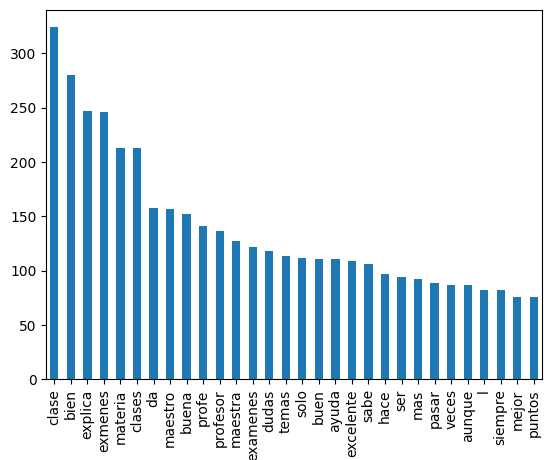
\includegraphics[width=0.8\textwidth]{frecuencia_palabras.png}
    \caption{Gráfico de frecuencias de palabras únicas en los comentarios de FCFM}
    \label{fig:frecuencia_palabras_unicas}
\end{figure}

\subsection{Análisis de Bigramas}

 Los bigramas, que son combinaciones de dos palabras consecutivas, proporcionaron información más detallada sobre los sentimientos expresados en los comentarios. Se observó que muchos de los bigramas reflejan un sentimiento positivo hacia los profesores y las materias.

\begin{figure}[h!]
    \centering
    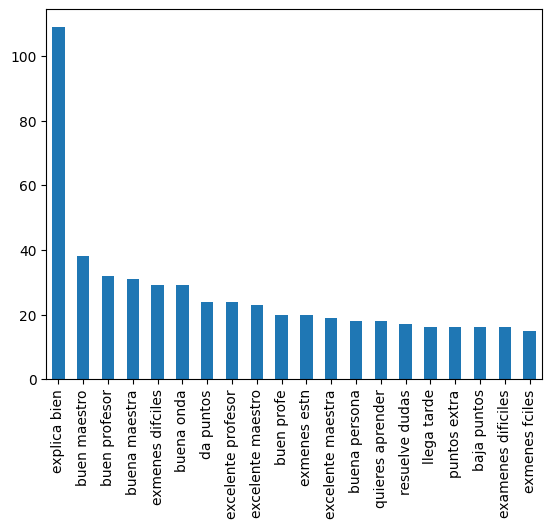
\includegraphics[width=0.8\textwidth]{frecuencia_bigramas.png}
    \caption{Gráfico de frecuencias de bigramas en los comentarios de FCFM}
    \label{fig:frecuencia_bigramas}
\end{figure}

\subsection{Análisis de Trigramas}

El análisis de trigramas, que considera combinaciones de tres palabras consecutivas, permitió identificarque los comentarios están relacionados con recomendaciones o advertencias sobre las actitudes y esfuerzos que los alumnos deben asumir durante el curso. La mayoría de los comentarios tienden a ser positivos, aunque condicionados a ciertas actitudes y comportamientos que los estudiantes deben adoptar para tener éxito en las materias.

\begin{figure}[h!]
    \centering
    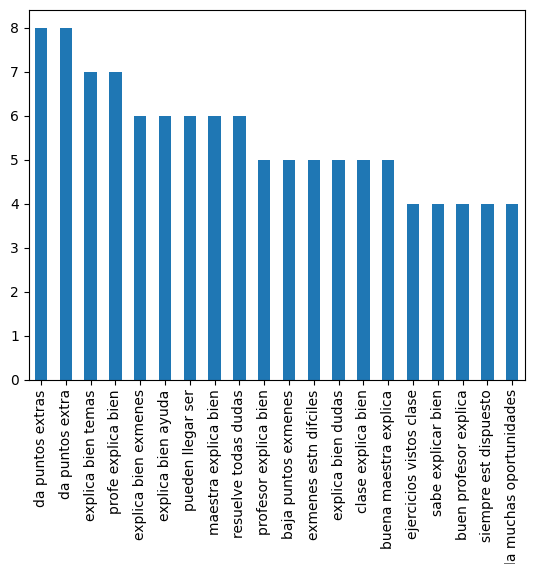
\includegraphics[width=0.8\textwidth]{frecuencia_trigramas.png}
    \caption{Gráfico de frecuencias de trigramas en los comentarios de FCFM}
    \label{fig:frecuencia_trigramas}
\end{figure}

\subsection{Interpretación General}

En resumen, los resultados del análisis indican que, si bien el uso de palabras únicas no proporciona una imagen clara del sentimiento general, la utilización de bigramas y trigramas permite una interpretación más precisa de los comentarios. A nivel general, los comentarios de los estudiantes sobre la FCFM son mayormente positivos. No obstante, es importante destacar que los estudiantes suelen condicionar sus comentarios a las actitudes y esfuerzos necesarios para superar los cursos con éxito. Este hallazgo sugiere que, aunque los profesores y las materias son bien valorados, los estudiantes reconocen la necesidad de un esfuerzo significativo para lograr buenos resultados académicos.

\subsection{Comparasión entre profesores}

\begin{figure}[h!]
    \centering
    \begin{subfigure}[b]{0.45\textwidth}
        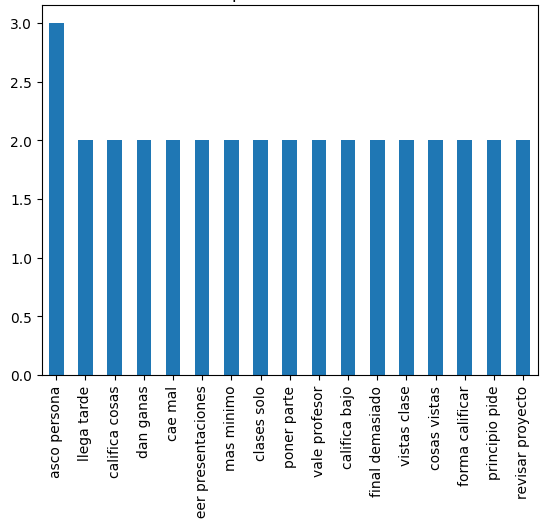
\includegraphics[width=\textwidth]{profe1.png}
        \caption{Profesor 1}
        \label{fig:profe1}
    \end{subfigure}
    \hfill
    \begin{subfigure}[b]{0.45\textwidth}
        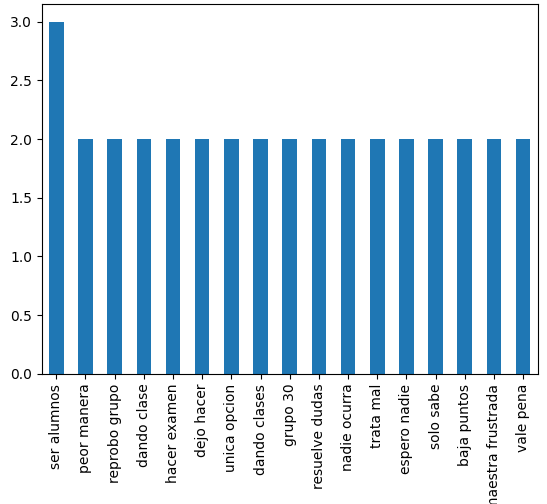
\includegraphics[width=\textwidth]{profe2.png}
        \caption{Profesor 2}
        \label{fig:profe2}
    \end{subfigure}

    \vspace{0.5cm} % Espacio vertical entre filas

    \begin{subfigure}[b]{0.45\textwidth}
        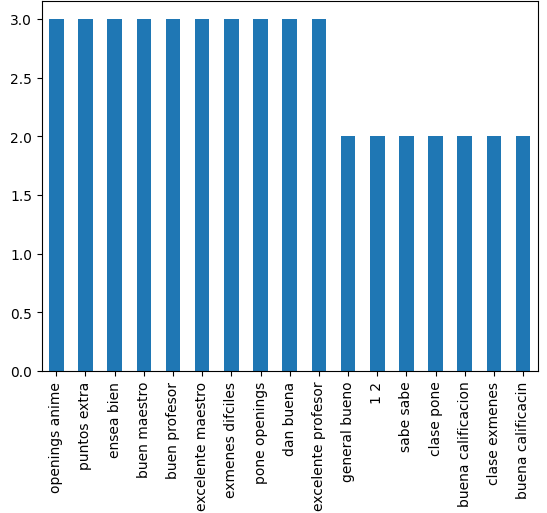
\includegraphics[width=\textwidth]{profe3.png}
        \caption{Profesor 3}
        \label{fig:profe3}
    \end{subfigure}
    \hfill
    \begin{subfigure}[b]{0.45\textwidth}
        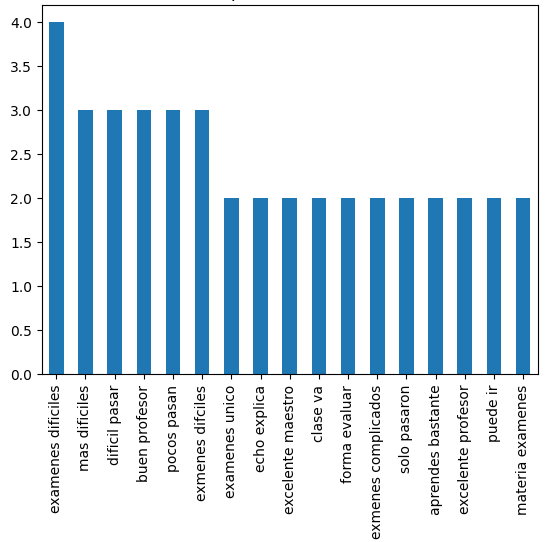
\includegraphics[width=\textwidth]{profe4.png}
        \caption{Profesor 4}
        \label{fig:profe4}
    \end{subfigure}
    \caption{Comparación de comentarios entre profesores}
    \label{fig:composicion_profe}
\end{figure}




Enseguida se revisarán los comentarios de cuatro maestros que tienen más comentarios para contrastar si el alumno considera al maestro como ideal para llevar el curso con él o ella. Para este caso, solo revisaremos bigramas:

\begin{itemize}
    \item \textbf{Profesor 1:} Por el conteo de frecuencia de palabras, vemos que el Profesor 1 ha sido mal evaluado, con comentarios predominantemente negativos.
    \item \textbf{Profesor 2:} De aquí se puede ver que el Profesor 2 cuenta con buenas evaluaciones. Sin embargo, encontramos características inesperadas en un maestro, como menciones a openings de anime. A nivel general, parece ser una buena opción para tomar clase con él.
    \item \textbf{Profesor 3:} El Profesor 3 cuenta con comentarios que explican que este es un profesor "difícil", pero un buen maestro. Esto resulta interesante, ya que una materia difícil no implica directamente un mal maestro.
    \item \textbf{Profesor 4:} El Profesor 4 cuenta con comentarios que explican que este es un profesor "fácil", que explica bien y que la materia resulta sencilla.
\end{itemize}

\subsection{Conclusión}
Los gráficos de frecuencias de las palabras utilizadas en los comentarios de la Facultad de Ciencias Físico Matemáticas (FCFM) a nivel general revelan que, aunque las palabras únicas no proporcionan una idea clara del tipo de sentimiento expresado en los comentarios, la aplicación de técnicas de análisis de bigramas y trigramas ofrece una comprensión más profunda de los comentarios positivos y negativos. A nivel general, los comentarios de los estudiantes tienden a ser positivos, aunque condicionados a ciertas actitudes y comportamientos que los estudiantes deben adoptar para tener éxito en las materias.

En conclusión, el análisis de frecuencias para texto nos permite interpretar los comentarios de una manera objetiva y comparable para tomar decisiones. En este ejemplo, mi opción de maestro, asumiendo que los cuatro maestros dieran la misma clase, sería el Profesor 3 porque es un buen maestro y permite llevar más allá la materia, haciéndola un poco difícil. Sin embargo, para un alumno que no le gusten los retos, optará por el Profesor 4, quien hace que su contenido sea mucho más sencillo o fácil.


%\section{Referencias}
 %   Lista de las referencias bibliográficas utilizadas en tu trabajo. Puedes utilizar el siguiente formato para las referencias en formato BibTeX.

%\begin{thebibliography}{9}
 %   \bibitem{Referencia1}
  %  Autor1, Autor2,
  %  \textit{Título del artículo o libro},
  %  Revista o Editorial,
   % Año.

    %\bibitem{Referencia2}
    %Autor1, Autor2,
    %\textit{Título del artículo o libro},
    %Revista o Editorial,
    %Año.
%\end{thebibliography}

\end{document}
